% !Mode:: "TeX:UTF-8"
%%%%%%%%%%%%%%%%%%%%%%%%%%%%%%%%%%%%%%%%%
% Thin Sectioned Essay
% LaTeX Template
% Version 1.0 (5/2/14)
%
% This template has been downloaded from:
% http://www.LaTeXTemplates.com
%
% Original Author:
% Nicolas Diaz (nsdiaz@uc.cl) with extensive modifications by:
% Vel (vel@latextemplates.com)
%
% Modifications by:
% Utopiar (Utopiar@gs.zzu.edu.cn) In ZZUNLP
%
% License:
% CC BY-NC-SA 3.0 (http://creativecommons.org/licenses/by-nc-sa/3.0/)
%
%%%%%%%%%%%%%%%%%%%%%%%%%%%%%%%%%%%%%%%%%

%----------------------------------------------------------------------------------------
%	引入支持包和文档设置
%----------------------------------------------------------------------------------------

\documentclass[a4paper, 11pt, hyperref, UTF8]{ctexart} % 字体大小 (可以设置为 10pt, 11pt or 12pt) and 纸张大小 (remove a4paper for US letter paper),汉语支持
%\documentclass[a4paper, 11pt]{article}

\usepackage[protrusion=true,expansion=true]{microtype} % Better typography
\usepackage{graphicx} % 图片包
\usepackage{wrapfig} % 允许图片或绕

\usepackage{float} %图片位置
\usepackage{amsmath} %公式
\usepackage{bm}  %加粗
\usepackage{CJK} %字体包

\usepackage[colorlinks,linkcolor=black,anchorcolor=black,citecolor=black]{hyperref}  %超链接包

\usepackage{mathpazo} % 使用Palatino字体
\usepackage[T1]{fontenc} % Required for accented characters
\linespread{1.05} % 更改行间距, Palatino字体默认改行最佳

\makeatletter
%\renewcommand\@biblabel[1]{\textbf{#1.}} % 更换引用序号'[1]' 为'1.'
\renewcommand{\@listI}{\itemsep=0pt} % 减少逐项列举项目之间的空间,并列举环境和参考书目

\renewcommand{\maketitle}{ % 自定义标题 - 在这里并不修改标题和作者的名字
\begin{flushleft} % 右对齐
{\LARGE\@title} % 加大标题字体

\vspace{50pt} % 标题和作者间的间距

{\large\@author} % 作者名格式
\\\@date % Date

\vspace{40pt} % 作者和摘要的距离
\end{flushleft}
}

%----------------------------------------------------------------------------------------
%	TITLE
%----------------------------------------------------------------------------------------

\title{\textbf{Logistic回归}\\ % Title
关于逻辑回归的读书笔记} % Subtitle

\author{\textsc{梁军} % Author
\\{\textit{郑州大学}}} % Institution

\date{\today} % Date

%----------------------------------------------------------------------------------------

\begin{document}
\maketitle % Print the title section
%----------------------------------------------------------------------------------------
%	ABSTRACT AND KEYWORDS
%----------------------------------------------------------------------------------------

%\renewcommand{\abstractname}{Summary} % Uncomment to change the name of the abstract to something else

\begin{abstract}
Logistic回归——我们经常用一条直线对一些点进行拟合(该线成为最佳拟合直线),这个拟合过程就称作回归。\cite{harrington2012machine}利用Logistic回归进行分类的主要思想是:根据现有数据对分类边界线建立回归公式,以此进行分类。Logistic回归的一般过程为:

\begin{enumerate}
\item 收集数据:采用任意方法收集数据。
\item 准备数据:由于需要进行距离计算,因此要求数据类型采用数值型。另外,结构话数据格式则最佳。
\item 分析数据:采用任意方法对数据进行训练。
\item 训练算法:大部分时间将用于训练,训练的目的是为了找到最佳的分类回归函数。
\item 测试算法:一旦训练步骤完成,分类将会很快。
\end{enumerate}

\end{abstract}

\hspace*{3,6mm}\textit{Keywords:} 机器学习 , 逻辑回归 , 最优化算法 % Keywords

\vspace{30pt} % Some vertical space between the abstract and first section

%----------------------------------------------------------------------------------------
%	ESSAY BODY
%----------------------------------------------------------------------------------------

\section{介绍}

好了,以上摘自机器学习实战这本书。写的有点抽象……看了这些,maybe一些童鞋对逻辑回归有那么一丢丢的理解,但一定还是不知其所以然,那么下面我们从回归、线性回归和逻辑方程来逐步深入逻辑回归:)
%--------------------------------------------------------------------------------------------
\subsection{神马是回归}
\paragraph{回归}按照我的理解就是有一堆数据,而且我们又事先知道这些数据之间的关系,举个例子说吧:比如我们知道弹簧的弹力与弹簧的形变量之间存在线性关系:F=kx,但是却不知道系数k的值,那么我们可以通过大量的弹力和与之对应的形变量来计算出弹性系数,这个过程就叫做回归。也就是说,在进行回归的时候我们首先要知道变量与因变量之间的关系,而仅仅是去计算参数集而已。可是现实中,我们往往对于数据之间的关系不得而知,这就需要去观察数据然后预测数据之间可能的关系,然后再去回归参数集。

当然,根据数据间的关系,我们可以将回归分为线性回归(一元一次方程、二元一次方程……)和非线性回归(N元M次方程、Log 方程、指数方程……)
%------------------------------------------------

\subsection{神马是线性回归}

\begin{figure}[H]
\centering
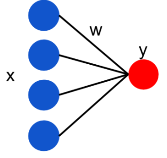
\includegraphics[width=0.38\textwidth,height=0.38\textwidth]{1.png}
\caption{线性回归}
\end{figure}
\paragraph{线性回归}我们举个最简单的例子,还是上面弹簧弹力与形变量之间的线性关系问题,它们之间是一元一次方程的关系,根据我们初中OR小学的知识我们可以知道:解这个方程仅仅需要一个F 值和一个与之对应的x值就OK 了,可是现实中由于这些数据都是测量出来的,不可避免的会出现误差甚至的错误,那么我们就需要大量数据来预测一个较为准确的弹性系数。通常采用的方式是,定义一个代价函数,通过最小化代价函数来估计参数集;或者定义代价函数为最大似然函数,通过最大化似然函数来估计参数集。


%------------------------------------------------


\subsection{神马是Logistic方程}

\begin{figure}[H]
\centering
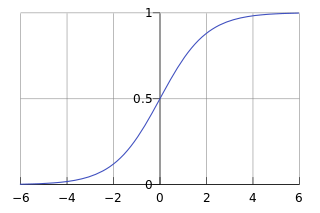
\includegraphics[width=0.38\textwidth,height=0.38\textwidth]{2.png}
\caption{Logistic方程}
\end{figure}
\paragraph{Logistic方程}——直觉上,一个线性模型的输出值 y 越大,这个事件$ P(Y=1|x) $ 发生的概率就越大。 另一方面,我们可以用事件的几率(odds)来表示事件发生与不发生的比值,假设发生的概率是 p ,那么发生的几率(odds)是 $p/(1-p) $, odds 的值域是 0 到正无穷,几率越大,发生的可能性越大。将我们的直觉与几率联系起来的就是下面这个(log odds)或者是 Logistic 函数 (有点牵强 - -!):
$$ Log\frac{p}{1-p} =  w^T \cdot x  $$

其中,$w$和$x$就为行向量。进而可以求出$p$关于$w \cdot x$的表示:
$$ P(Y=1|x)  = \frac{e^{w^T \cdot x}}{1+e^{w^T \cdot x}}$$

看到这里,恭喜你!终于见到传说中的Logistic函数了,其实就是人为的将线性回归的结果与对数概率结合在了一起!以$w \cdot x$为自变量的函数图2所示。

我们可以看得出,当横坐标拉伸时,该函数图像就像是一个阶跃函数一样,因此可以用它来做分类!
%---------------------------------------------------

\section{参数估计方法}

上面也简单提到了一下,对于回归我大致了解到的有两种参数估计方法:
\begin{enumerate}
\item 最大似然估计法
\item 平方损失函数估计法
\end{enumerate}

\subsection{最大似然法}

逻辑回归输出的是分到每一类的概率,参数估计的方法自然可以用最大似然估计 (MLE) 咯。对于训练样本来说,假设每个样本是独立的,输出(标签)为 $y = {0, 1}$,样本的似然函数就是将所有训练样本 label 对应的输出节点上的概率相乘, 令 $p = P(Y=1|x)$ ,如果 $y = 1$, 概率就是$ p$, 如果 $y = 0$, 概率就是$ 1 - p $,(好吧,我是个罗嗦的家伙),  将这两种情况合二为一,得到似然函数:
$$ L=\prod_{i=1}^{N}{[P(Y=1|x_i)]^{y_i} [P(Y=0|x_i)]^{1-y_i}} $$
有连乘,这个好办,取对数就OK:

\begin{align*}
 L(w) &= \sum _{i=1} ^{N} {y^i log(P(Y=1|x_i)) + (1-y^i)log(P(Y=0|x_i))} \\
      &= \sum _{i=1} ^{N} {y^i log(P(Y=1|x_i)) + log(P(Y=0|x_i)) - y^ilog(P(Y=0|x_i))} \\
      &= \sum _{i=1} ^{N} {y^i log\frac{P(Y=1|x_i)} {P(Y=0|x_i)} + log(P(Y=0|x_i))} \\
\end{align*}
根据上面的对数概率公式,我们可以得到:
$$ L(w) = \sum _{i=1} ^{N} {y^i (\vec w^T \cdot \vec x ) - log(1 + e^{w^T \cdot x})}$$
对$w$求导可以得到:
$$ \frac {\partial L(w)}{\partial w} = \sum _{i=1} ^{N} {y_ix} - \sum_{i=1}^{N}{\frac{e^{w^Tx}}{1+e^{w^Tx}}x} = \sum _{i=1} ^{N} {(y_i - P(Y=1|x))x}$$

\subsection{平方损失函数法}

\paragraph{平方损失函数}通常在定义了一个模型($f(x;w_0,w_1)=w_0+w_1x$)之后,衡量一个特定模型与数据点接近程度的普遍方法是真实值与模型预测值之间的平方差\cite{rogers2011first}。平方差可以定义为:

$$ {(t_n - f( x_n; w_0, w_1 ))}^2 $$
这个表达式就称之为\textbf{平方损失函数}。

如果$ f(x_n; w_0, w_1) $仅是一个线性模型,那么该方法就是用于线性回归的参数拟合;但是在$ f(\cdot) $外层加上激活函数Logistic函数,那么该方法就是用于逻辑回归的参数拟合。由此,我们可以看出,从线性模型到逻辑模型仅仅是在线性函数外层嵌套一个Logistic函数而已,那么我们不禁要问什么时候使用线性模型,什么时候使用逻辑模型呢?根据我的理解,这个需要依据已有数据的结果集来判断:

\begin{enumerate}
\item 当结果集中属于二分类问题时,一般选用逻辑模型。
\item 当结果集中为连续型预测值时,一般选用线性模型。
\end{enumerate}

对于整个数据集,考虑其平均损失,即:

$$ \pounds_n(t_n, f(x_n; w_0, w_1)) = (t_n - f(x_n; w_0, w_1))^2 $$

$$ \pounds = \frac{1}{N} \sum_{n=1}^{N}{\pounds_n(t_n, f(x_n; w_0, w_1))}$$
$\pounds$就是我们要定义的损失函数,为了得到更符合实际的参数集,我们当然希望损失函数越小越好。因此,我们需要根据数据集调整$w_0$和$w_1$来产生一个模型,词模型得到平均损失的最低值。使用数学表达式可以表示为:

$$ \arg \min_{w_0,w_1}\frac{1}{N} \sum_{n=1}^{N}{\pounds_n(t_n, f(x_n; w_0, w_1))} $$
argmin项是数学上“找到最小化参数”的缩写,即“argument of the minimum”,这个曾经也是困惑了笔者好久,o(╯□╰)o

\begin{align*}
\pounds &= \frac{1}{N} \sum_{n=1}^{N}{\pounds_n(t_n, f(x_n; w_0, w_1))} \\
        &= \frac{1}{N} \sum_{n=1}^{N}{(t_n - f(x_n; w_0, w_1))}^2 \\
        &= \frac{1}{N} \sum_{n=1}^{N}{(t_n - (w_0 + w_1x_n))}^2 \\
        &= \frac{1}{N} \sum_{n=1}^{N}{(w_1^2x_n^1+2w_1x_n(w_0-t_n)+w_0^2-2w_0t_n+t_n^2)}
\end{align*}
然后对于损失函数$\pounds$分别关于$w_0$和$w_1$求导,令得到的偏导数等于0,求出$w_0$和$w_1$的表达式:
$$ \widehat{w_0} =  \bar{t} - w_1\bar{x}$$
$$ \widehat{w_1} = \frac{\bar{xt} - \bar{x}\bar{t}}{\bar{x^2} - (\bar{x})^2} $$
对于该例中仅有两个参数$w_0$和$w_1$,该方法还可以使用,但如果有成百上千个参数呢?如此做法,一定会令你痛不欲生:(

事实上,我们一般采用矩阵的形式来表示,首先我们做如下约定:使用黑体表示矩阵或者向量,矩阵用大写字母表示,向量用小写字母表示,并且所有向量均为行向量,列向量使用行向量的转置表示。那么,我们定义$\bm{w}$表示参数向量,$\bm{x_i}$表示第i个数据集的特征向量,$\bm{X}$表示整个数据集的特征向量,$\bm{t}$表示结果向量集。那么,代价函数可以表示为:

\begin{align*}
\ \pounds &= \frac{1}{N}(\bm{t}-\bm{Xw}^T)^T(\bm{t}-\bm{Xw^T}) \\
          &= \frac{1}{N}(\bm{t}^T\bm{t} - \bm{t}^T\bm{X}\bm{w}^T - \bm{w}\bm{X}^T\bm{t}+\bm{w}\bm{X}^T\bm{X}\bm{w}^T) \\
          &= \frac{1}{N}(\bm{t}^T\bm{t} - 2\bm{w}\bm{X}^T\bm{t}+\bm{w}\bm{X}^T\bm{X}\bm{w}^T) \\
\end{align*}
根据向量微分的求导规则:
\begin{center}
\begin{tabular}{c|c}
\hline
$f(w)$                 & $\frac{\partial{f}}{\partial{w}}$   \\
\hline
$\bm{w}^T\bm{x}$       & $\bm{x}$                            \\
%\hline
$\bm{x}^T\bm{w}$       & $\bm{x}$                            \\
%\hline
$\bm{w}^T\bm{w}$       & $2\bm{w}$                           \\
%\hline
$\bm{x}^T\bm{C}\bm{w}$ & $2\bm{Cx}$                          \\
\hline
\end{tabular}
\end{center}
得到:
$$ \frac{\partial{\pounds}}{\partial{w}} = \frac{2}{N}\bm{X}^T\bm{Xw}-\frac{2}{N}\bm{X}^T\bm{t} $$
%------------------------------------------------

\section{最优化算法}

我们可以采用梯度下降算法。(未完待续……)


%----------------------------------------------------------------------------------------
%	BIBLIOGRAPHY
%----------------------------------------------------------------------------------------

%\begin{thebibliography}{0}

%\bibitem{Harrington2012}
%Harrington, Peter. \emph{Machine Learning in Action}. Manning Publications Co., 2012.

%\bibitem{Rogers2011}
%Rogers, Simon, and Mark Girolami. \emph{A first course in machine learning}. CRC Press, 2011.

%\bibitem{zouxy092014}
%zouxy09. \emph{\href{http://blog.csdn.net/zouxy09/article/details/20319673}{机器学习算法与Python实践之(七)逻辑回归(Logistic Regression)}}.  CSDN, 2014.

%\bibitem{Su2011}
%苏冉旭. \emph{\href{http://hi.baidu.com/hehehehello/item/40025c33d7d9b7b9633aff87}{逻辑回归概述}}. 百度, 2011.

%\bibitem{daniel-D2013}
%daniel-D.  \emph{\href{http://www.cnblogs.com/daniel-D/archive/2013/05/30/3109276.html}{Logistic Regression 之基础知识准备}}. cnblog, 2013.
%\end{thebibliography}

%-------------------------------------------------------------------------------------------------------
%使用bibtex文件
%-------------------------------------------------------------------------------------------------------

\bibliographystyle{unsrt}

\bibliography{Rogers}
%-------------------------------rogers2011first---------------------------------------------------------
\end{document}
